%%%%%%%%%%%%
%
% $Autor: Wings $
% $Datum: 2019-03-05 08:03:15Z $
% $Pfad: Troubleshooting.tex $
% $Version: 4250 $
% !TeX spellcheck = en_GB/de_DE
% !TeX encoding = utf8
% !TeX root = manual 
% !TeX TXS-program:bibliography = txs:///biber
%
%%%%%%%%%%%%

\chapter{Troubleshooting}

If you encounter issues while using the Hurricane Intensity Prediction System, follow the steps below to identify and resolve common problems. This approach will help ensure smooth operation and reliable predictions.

\begin{figure}[h]
	\centering
	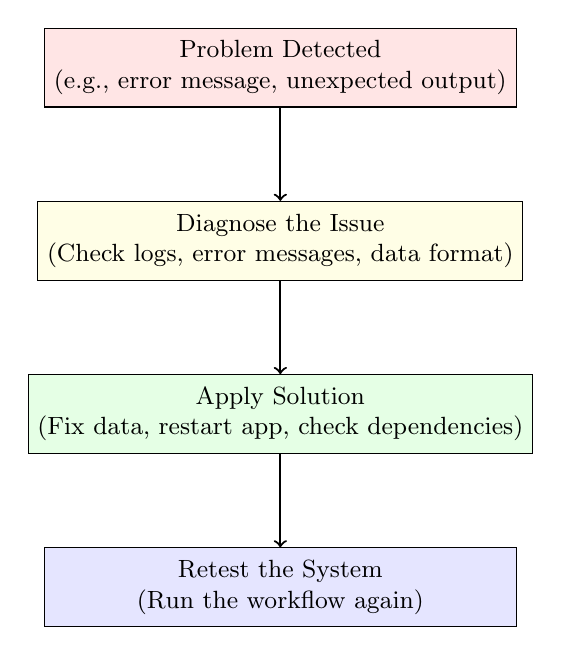
\begin{tikzpicture}[node distance=2.2cm, every node/.style={rectangle, draw, minimum width=6cm, minimum height=1cm, align=center, font=\small}]
		\node[fill=red!10] (error) {Problem Detected\\(e.g., error message, unexpected output)};
		\node[below of=error, fill=yellow!10] (diagnose) {Diagnose the Issue\\(Check logs, error messages, data format)};
		\node[below of=diagnose, fill=green!10] (solution) {Apply Solution\\(Fix data, restart app, check dependencies)};
		\node[below of=solution, fill=blue!10] (retest) {Retest the System\\(Run the workflow again)};
		
		\draw[->, thick] (error) -- (diagnose);
		\draw[->, thick] (diagnose) -- (solution);
		\draw[->, thick] (solution) -- (retest);
	\end{tikzpicture}
	\caption{Troubleshooting Workflow for the Hurricane Intensity Prediction System}
\end{figure}

\section*{Common Issues and Solutions}

\begin{itemize}
	\item \textbf{Application Fails to Start:} \\
	Ensure all required Python packages are installed. Run \texttt{pip install -r requirements.txt} in your terminal.
	
	\item \textbf{File Upload Not Working:} \\
	Verify that your data file is in the correct format (e.g., CSV with columns for date, time, location, wind speed, pressure). Check for missing or malformed values.
	
	\item \textbf{No Predictions Generated:} \\
	Confirm that the \texttt{models/} directory contains the pre-trained ARIMA and LSTM model files. If missing, contact the developer to retrain and save the models.
	
	\item \textbf{Incorrect or Unexpected Predictions:} \\
	Double-check your input data for accuracy and completeness. Outliers or missing values can affect model performance.
	
	\item \textbf{Visualization Not Displayed:} \\
	Make sure your browser supports interactive plots and that there are no errors in the Streamlit app logs.
	
	\item \textbf{Permission or Access Errors:} \\
	Ensure you have the necessary permissions to read/write files in the project directory, especially for uploading data and downloading results.
	
	\item \textbf{Other Errors:} \\
	Review any error messages shown in the app or terminal. Consult the FAQ or contact support if the problem persists.
\end{itemize}

\textbf{Tip:}  
If you encounter persistent issues, restarting the Streamlit app and re-uploading your data can often resolve temporary glitches.

\textbf{Note:}  
For critical or unresolved problems, please contact the system administrator or developer for further assistance.










